
%(BEGIN_QUESTION)
% Copyright 2010, Tony R. Kuphaldt, released under the Creative Commons Attribution License (v 1.0)
% This means you may do almost anything with this work of mine, so long as you give me proper credit

A process used in the oil refining industry to make high-octane gasoline feedstock is called {\it alkylation}.  So-called ``alky'' units employ a concentrated acid as the catalyst for the alkylation reaction, usually sulfuric acid:

$$\includegraphics[width=15.5cm]{i04515x01.eps}$$

The ``acid settler'' vessel is a separator, allowing the reaction products and acid catalyst to separate according to their respective densities (concentrated sulfuric acid being denser than any hydrocarbon).  The interface level between hydrocarbon liquid and acid must be tightly controlled for the process to work well.  It is bad for acid to ``carry over'' to the caustic scrubber (if the interface rises too high), and it is also bad for hydrocarbon liquids to leave the system through the ``reject acid'' line (if the interface falls too low).

\vskip 10pt

Research typical permittivity values for hydrocarbon liquids and sulfuric acid, then calculate the reflection factor ($R$) for the hydrocarbon/acid interface assuming the use of a guided-wave radar instrument to measure this oil/acid interface level.  

\vskip 20pt \vbox{\hrule \hbox{\strut \vrule{} {\bf Suggestions for Socratic discussion} \vrule} \hrule}

\begin{itemize}
\item{} What types of {\it personal protective equipment} (PPE) do you think an instrument technician might need to wear before working on a instrument contacting this highly concentrated acid?
\end{itemize}

\underbar{file i04515}
%(END_QUESTION)





%(BEGIN_ANSWER)

$R \approx$ 28.8\%

%(END_ANSWER)





%(BEGIN_NOTES)

This value for $R$ was calculated using $\epsilon_{oil}$ = 2 and $\epsilon_{acid}$ = 22.

%INDEX% Measurement, interface level: radar
%INDEX% Process: petroleum alkylation 

%(END_NOTES)

